% Checked with Grammarly - 22/03/2021

\chapter{Results and Evaluation}

\section{Data Collection}

The VisiBot Processing System was deployed over a five-week (35-day) data collection period between 11/02/2021 and 11/03/2021, resulting in the processing and analysis of 61,293 honeypot packets collected from various strategically located honeypot servers hosted by Bad Packets. As the deployed honeypots mimic that of IoT device characteristics, the proposed system was able to identify multiple IoT botnets, including several prominent Peer-to-Peer botnets. Throughout the deployment period, a 3-worker LiSa Sandbox server was hosted on a separate network from the VisiBot Processing System, ensuring a separation of concerns. All objects generated during malware analysis, such as malware samples, program output logs, and packet capture (pcap) files, were actively stored on a secure block-storage partition. The block-storage partition ensures that if the sandbox were to become compromised, the server could be safely reset without presenting a loss of valuable information. Throughout the collection process, the LiSa sandbox operated using three celery workers and executed all binaries for a total of 30 seconds. Additionally, the VisiBot was configured to use six celery workers to allow for parallelised processing of honeypot data and LiSa analysis reports.

Following the analysis of 61,293 honeypot packets, VisiBot lead to the identification of 58,010 unique public IP addresses, including 1,303 candidate Command \& Control servers and 6,876 P2P Nodes. Additionally, the system logged 4,000 Autonomous Systems, 82,050 botnet events, and extracted 9,923 malware payload URLs. Out of the payload URLs extracted, a total of 1,654 malware samples were successfully retrieved, consisting of a total of 150 unique MD5 hashes. Following malware analysis of all extracted samples via the VirusTotal aggregation service, a total of 62,203 out of 97,659 anti-virus vendor scans were positive. Throughout the data collection period, all significant honeypot and malware traffic was classified into a total of six categories using a combination of packet analysis and heuristic analysis techniques. The categorised distribution of all traffic processed by VisiBot is highlighted below: 

\begin{figure}[!htb]
    \centering
    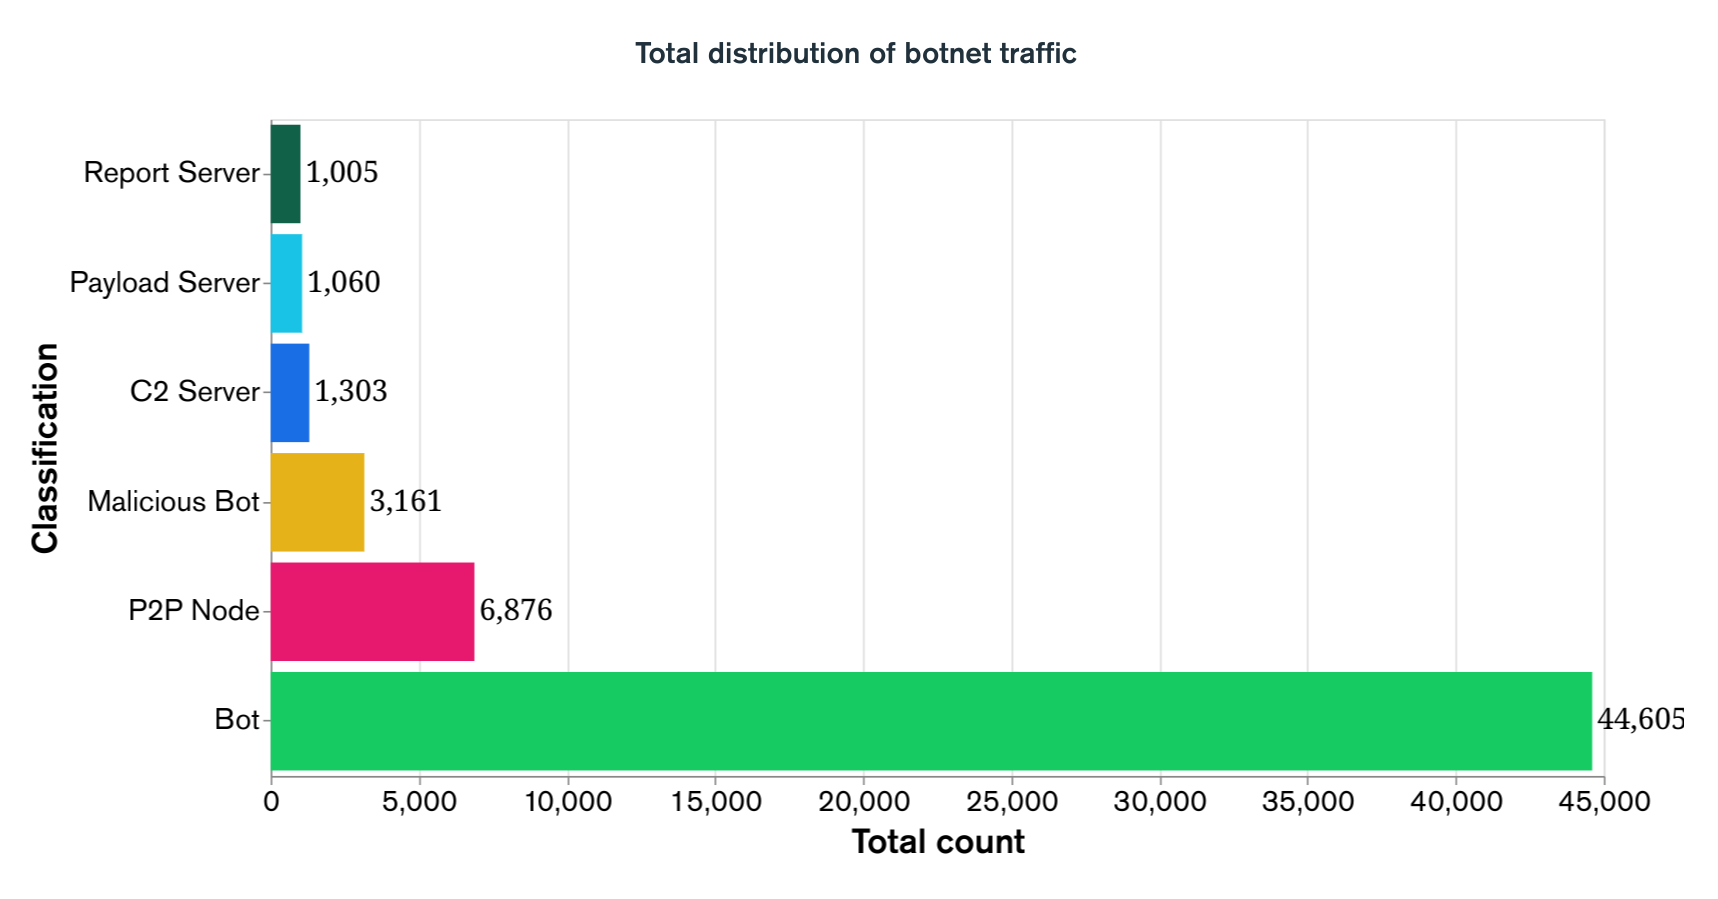
\includegraphics[width=0.75\linewidth]{results/botnet_distribution_histogram.png}
    \caption{distribution of classified botnet traffic.}
    \label{fig:botnet_distribution} 
\end{figure}

\newpage

Despite a significant proportion of detected botnet traffic being that of benign Mirai-like port-scanning activity, a large proportion of traffic has been observed to originate from several Peer-to-Peer networks and malicious (self-propagating) bots. Notably, more malicious bots have been observed than Report Servers and Payload Servers, which are commonly observed across centralised Mirai botnets. This may allude to a potential change in contemporary botnet propagation strategies, as bots are now being utilised to self-host malware and actively perform Remote Code Execution attacks. However, as this type of activity is most commonly associated with Peer-to-Peer IoT botnets like Hajime, the above graph may reflect a recent transition from previously accepted centralised botnets to highly dominant de-centralised Peer-to-Peer botnets.

\section{Geographic Botnet Distribution}

Throughout the five-week automated processing period, Visibot collected a wide array of IP address metadata, including geographic and autonomous system information. Such data includes the city, country, and continent of all IP addresses encountered, as well as geographic coordinates sourced from a frequently updated MaxMind GeoIP2 database. The broker-based detection system successfully processed and classified a multitude of honeypot packets, encountering activity spanning several continents, including Europe, North America, South America, and Asia. The geographic metadata of identified botnet entities can be analysed to better understand how IoT botnets are currently propagating. Additionally, geographic analysis allows for the visualisation of botnet growth and geographic IoT botnet hot-spots. The below heat-map visualises geographic botnet density through the plotting of latitude and longitude coordinates collected during analysis. Areas of high botnet traffic density are represented using a yellow-red colour gradient, whereas diminished areas are represented as opaque green-blue gradients:

\begin{figure}[!htb]
    \centering
    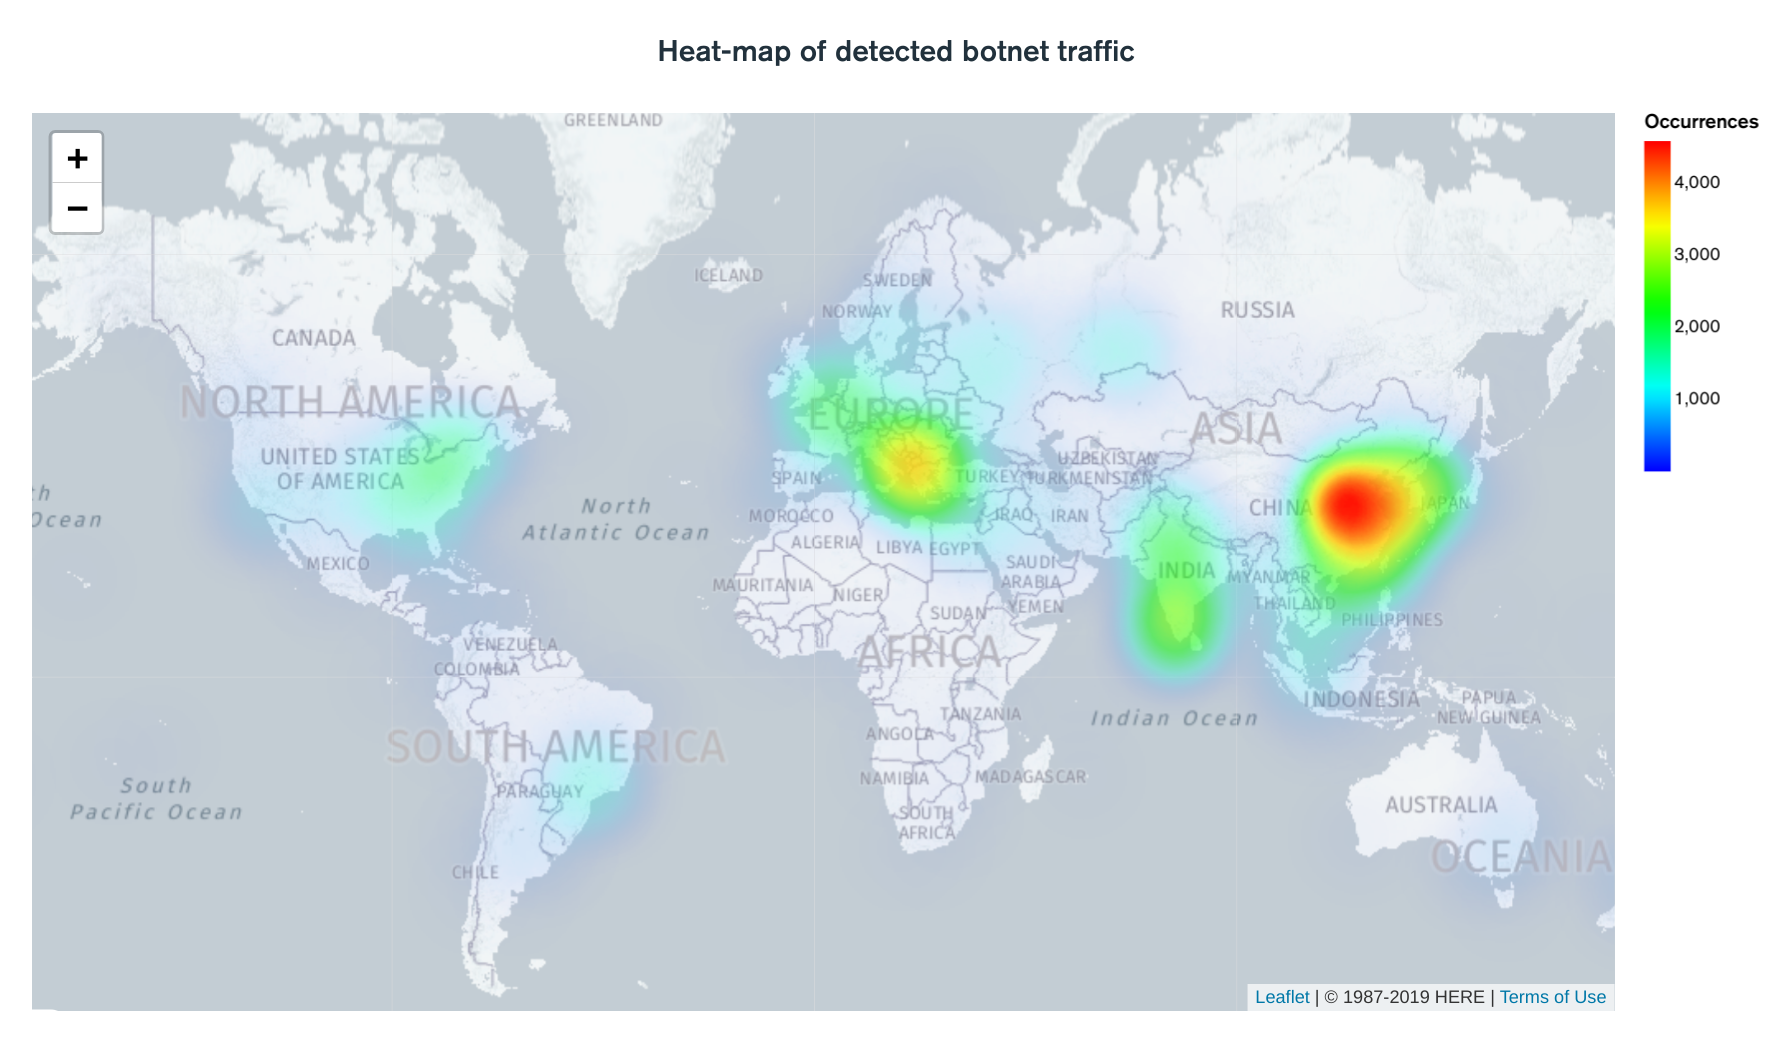
\includegraphics[width=0.8\linewidth]{results/all_heatmap.png}
    \caption{Geographic distribution of all botnet traffic detected by the VisiBot Processing System.}
    \label{fig:overall_heatmap} 
\end{figure}

The above geographic analysis indicates significant traffic density originating from various regions. However, the density of botnet traffic originates from Asia, where China is highlighted as the largest region. As inferred by the traffic distribution histogram previously shown in Figure \ref{fig:botnet_distribution}, a vast proportion of all traffic originating from China is that of Mirai-like port-scanning activity. Given that China is one of the leading countries for manufacturing IoT devices, and many of which have security vulnerabilities, it is likely that the quantity of IoT devices hosted in china has resulted in the country becoming an IoT botnet hot-spot. Similar but less significant geographic density patterns are also observed across India, Europe, North America, and Brazil. However, when comparing the geographic distribution of identified Command \& Control candidates and Peer-to-Peer nodes, several differences can be observed when compared to the overall botnet density map. Consider the below side-by-side comparison of the geographic density of all candidate C2 servers and P2P nodes identified by VisiBot:

\begin{figure}[!htb]
    \centering
    \subfloat[\centering Candidate C2 Server Geographic Distribution]{{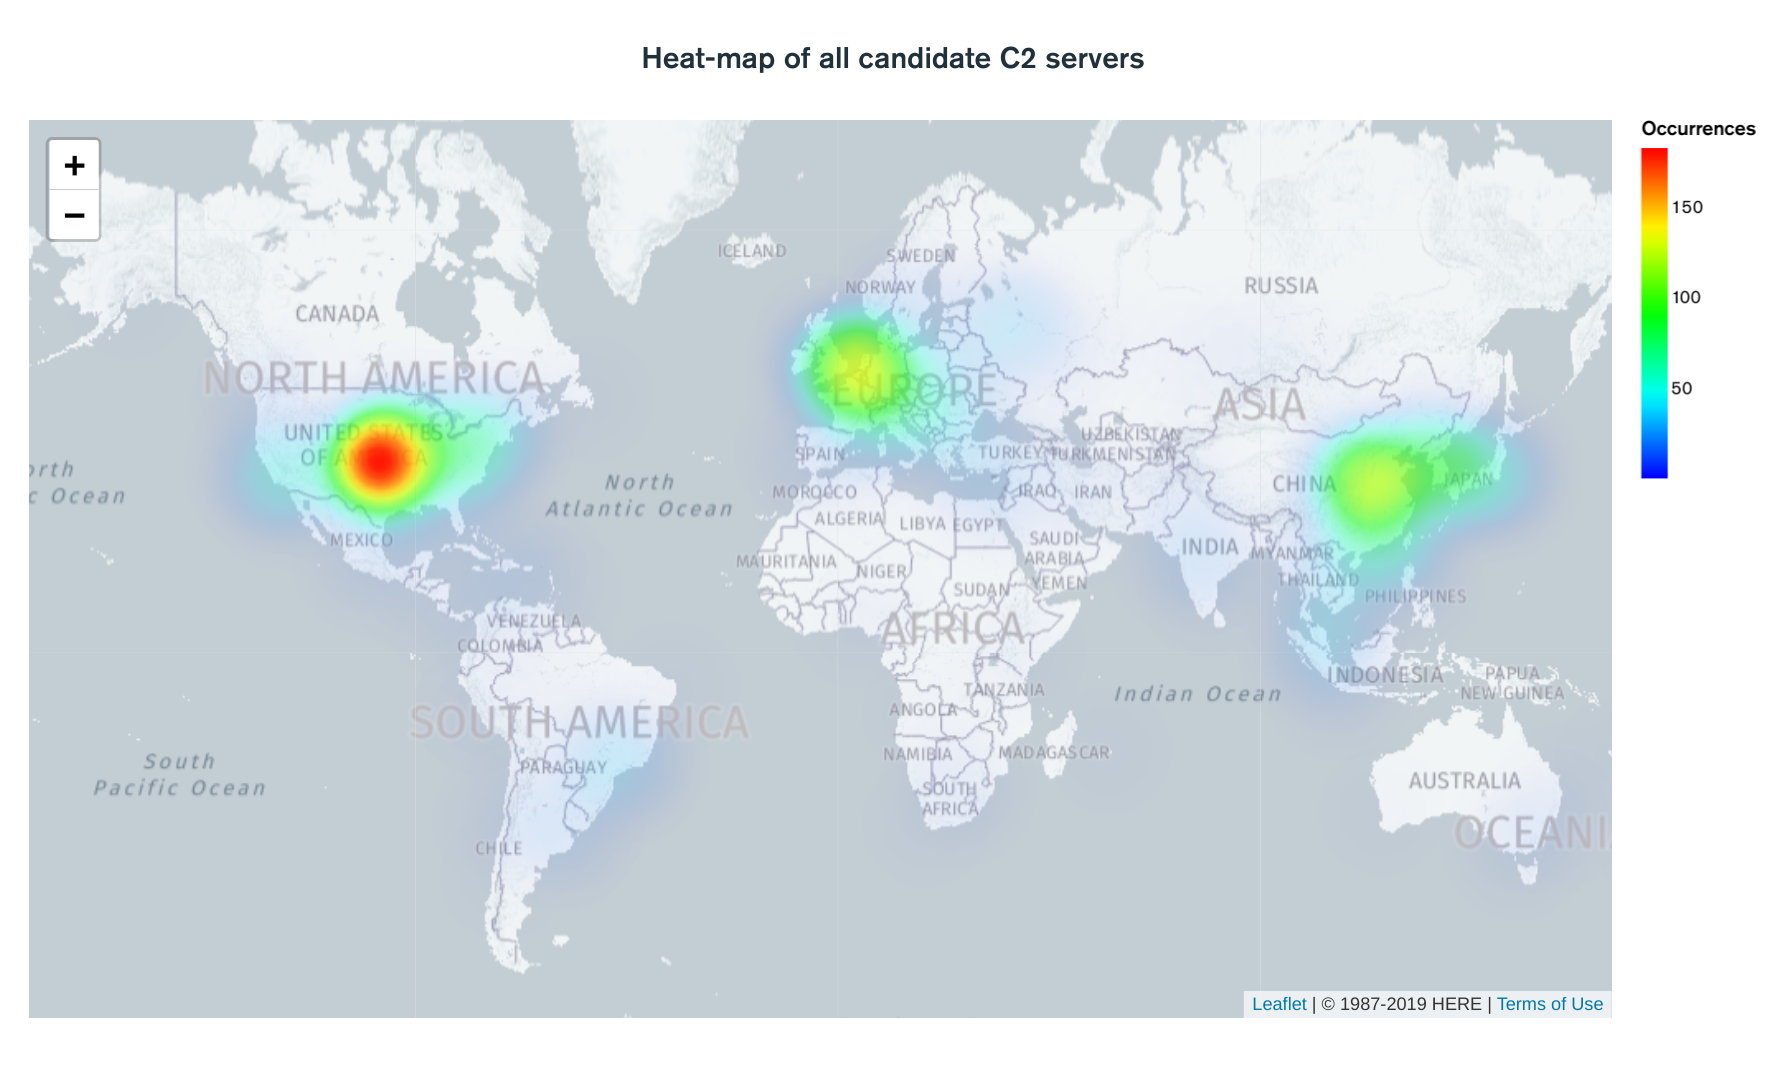
\includegraphics[width=6cm]{results/c2_heatmap.png} }}
    \qquad
    \subfloat[\centering P2P Node Geographic Distribution]{{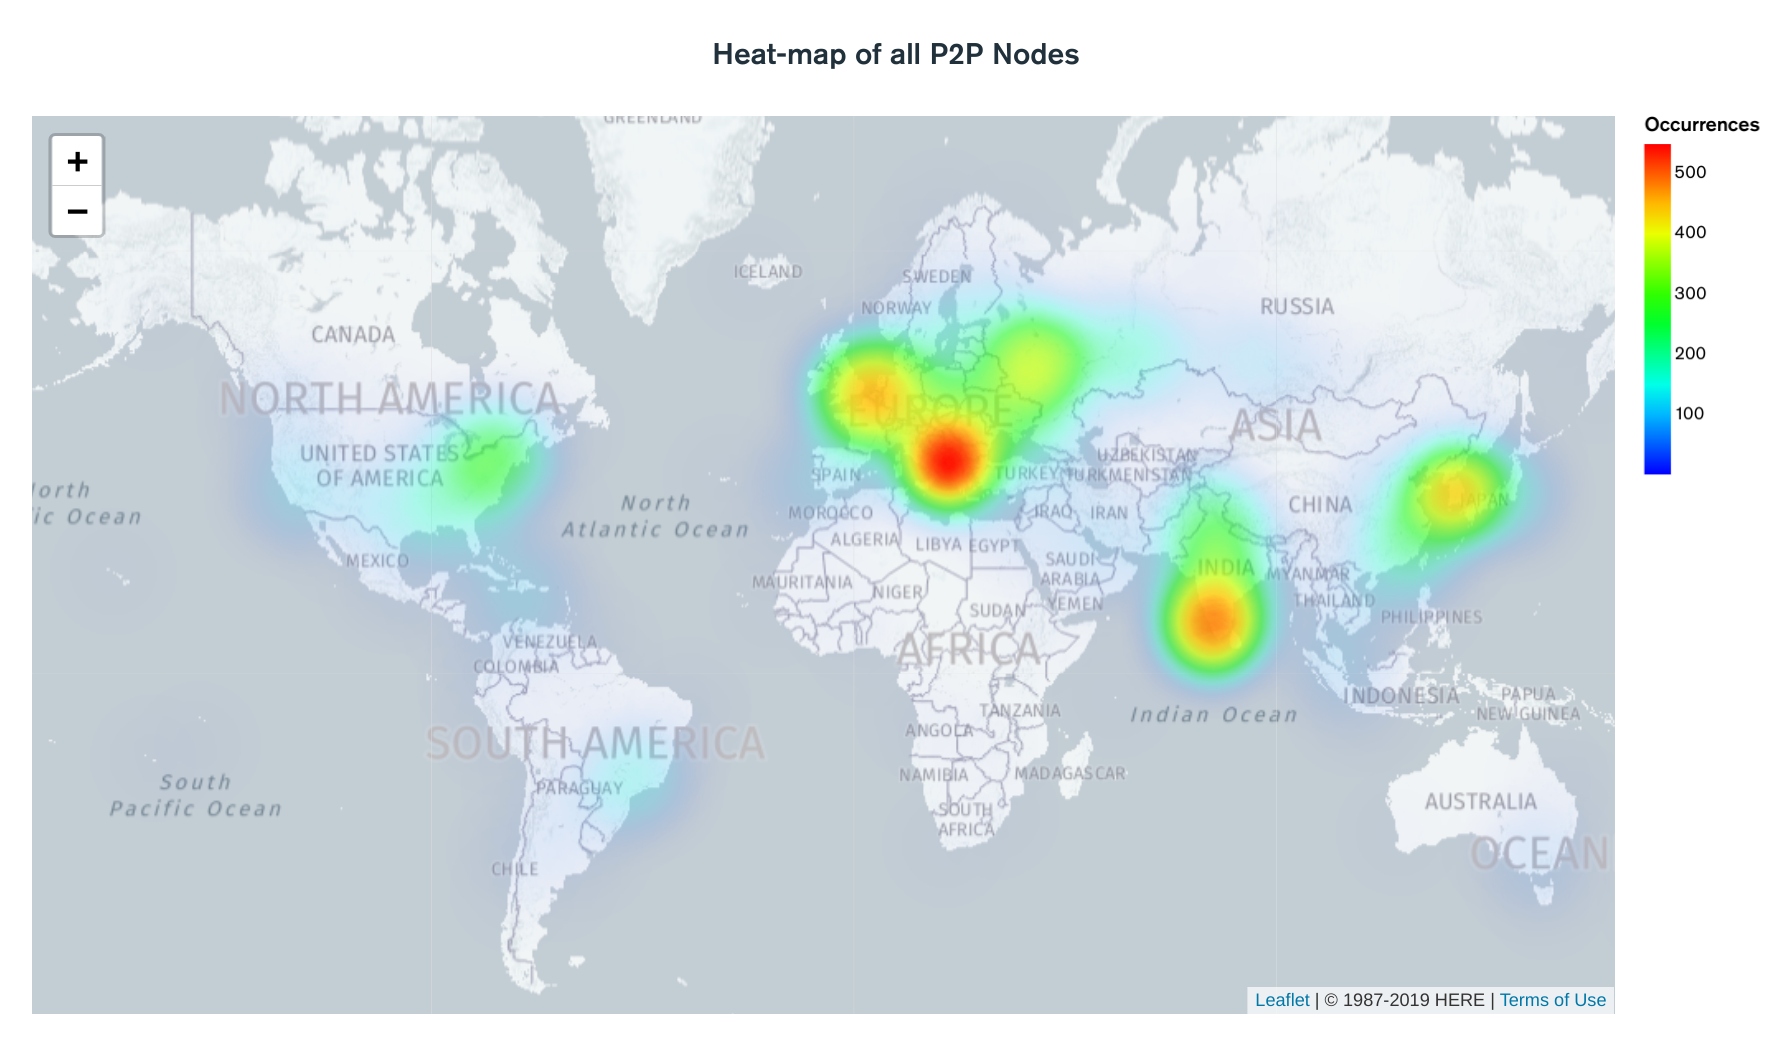
\includegraphics[width=6cm]{results/p2p_heatmap.png} }}
    \caption{Malware sample architecture and endianness represented side by side.}
    \label{fig:p2p_c2_heatmaps}
\end{figure}

As shown, the heat-map visualisation of candidate Command \& Control server distribution shows very high botnet activity across the United States of America. Medium C2 density is also observed across Europe and China. There is a clear contrast in traffic distribution when comparing geographic C2 density against all botnet traffic. The high level of C2 activity originating from North America indicates that most globally distributed botnets are being controlled by servers or computer systems located in the United States, with some occurrences logged in Central Europe and China. Adversely, most identified Peer-to-Peer botnet traffic is highly prevalent amongst Central Europe and India, with a wider global distribution than Candidate C2 Servers. As Peer-to-Peer botnets operate through communicating with peer nodes, which are often distributed across several countries and continents, a wide geographical distribution can be observed. In contrast, C2 servers often only operate out of specific regions, which are in some cases local to the botmaster. The distinction between the geographic distribution of overall, C2, and P2P traffic is further highlighted when inspecting the distribution of associated Autonomous System registries:

\begin{figure}[!htb]
    \centering
    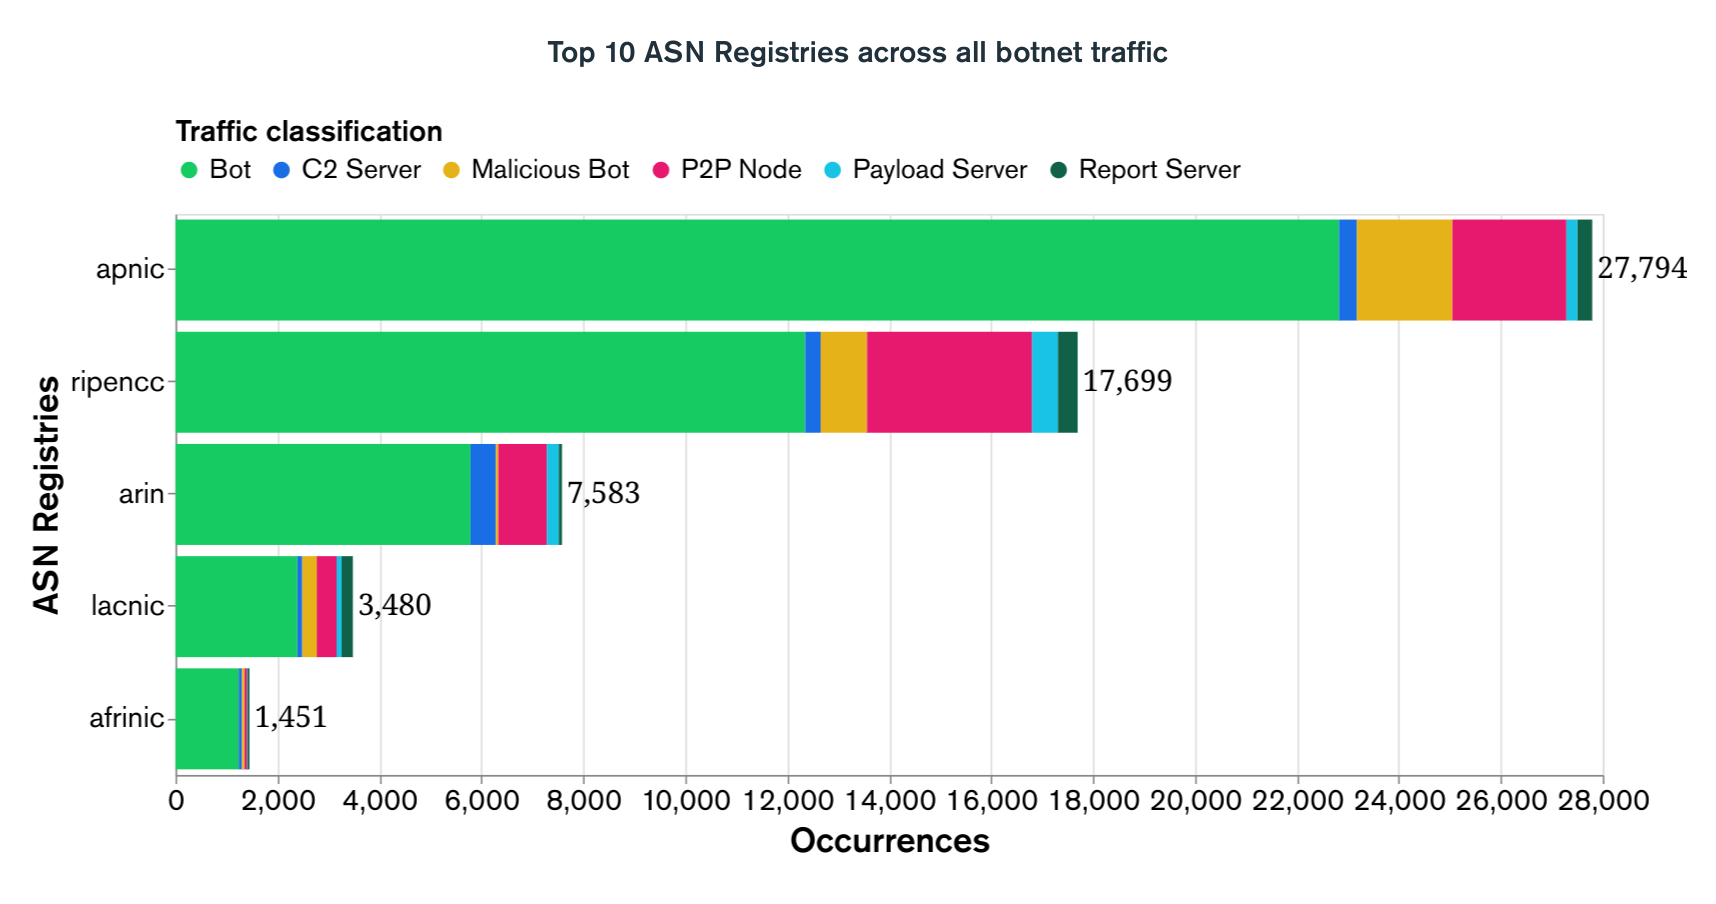
\includegraphics[width=0.9\linewidth]{results/top_ASN_registries.png}
    \caption{distribution of classified botnet traffic across ASN registries.}
    \label{fig:asn_registries_barchart} 
\end{figure}

Both the APNIC and RipeNCC ASN registries are widely associated with Mirai-like scanning, malicious botnet, and Peer-to-Peer activity. The bulk of identified port-scanning, malicious, and Peer-to-Peer botnet activity originates from IP addresses provided by Autonomous Systems operating within Asia-Pacific and Central/Eastern Europan regions. Adversely, the ARIN registry is more frequently associated with candidate C2 traffic and Peer-to-Peer traffic, with little occurrence of a malicious bot, report server or payload server activity seen across the United States, Canada, and North Atlantic. These findings are further validated by measuring the distribution of Autonomous Systems based on their country of origin:

\begin{figure}[!htb]
    \centering
    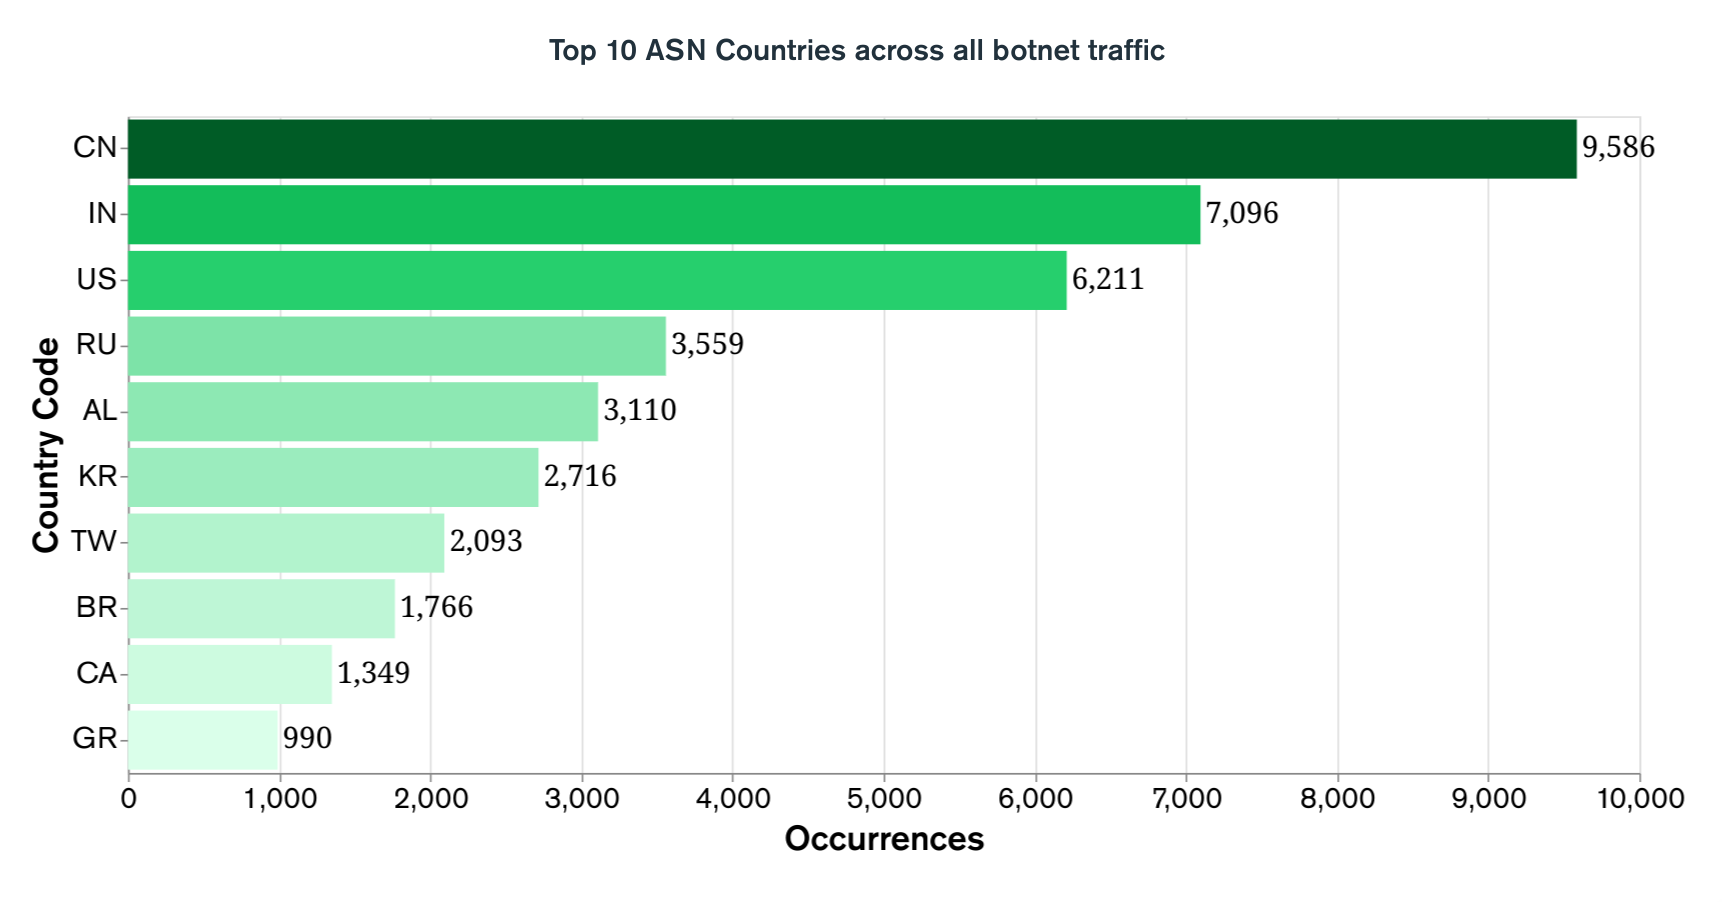
\includegraphics[width=0.75\linewidth]{results/top_10_asn_countries_overall.png}
    \caption{Top 10 ASN country codes for overall botnet traffic.}
    \label{fig:overall_asn_country_barchart} 
\end{figure}

As inferred in Figure \ref{fig:overall_heatmap}, the above graph confirms that the leading country of origin for overall botnet traffic is indeed China, followed by India, the United States, and Russia. Using this information, we can deduce that IoT device traffic originating from China is primarily that of port-scanning and malicious bot activity. However, when inspecting the geographic distribution of ASNs associated with C2 or P2P botnet traffic, the origin of such traffic differs significantly from the geographic distribution of overall traffic:

\begin{figure}[!htb]
    \centering
    \subfloat[\centering Top 10 Candidate C2 Server ASN Country Codes ]{{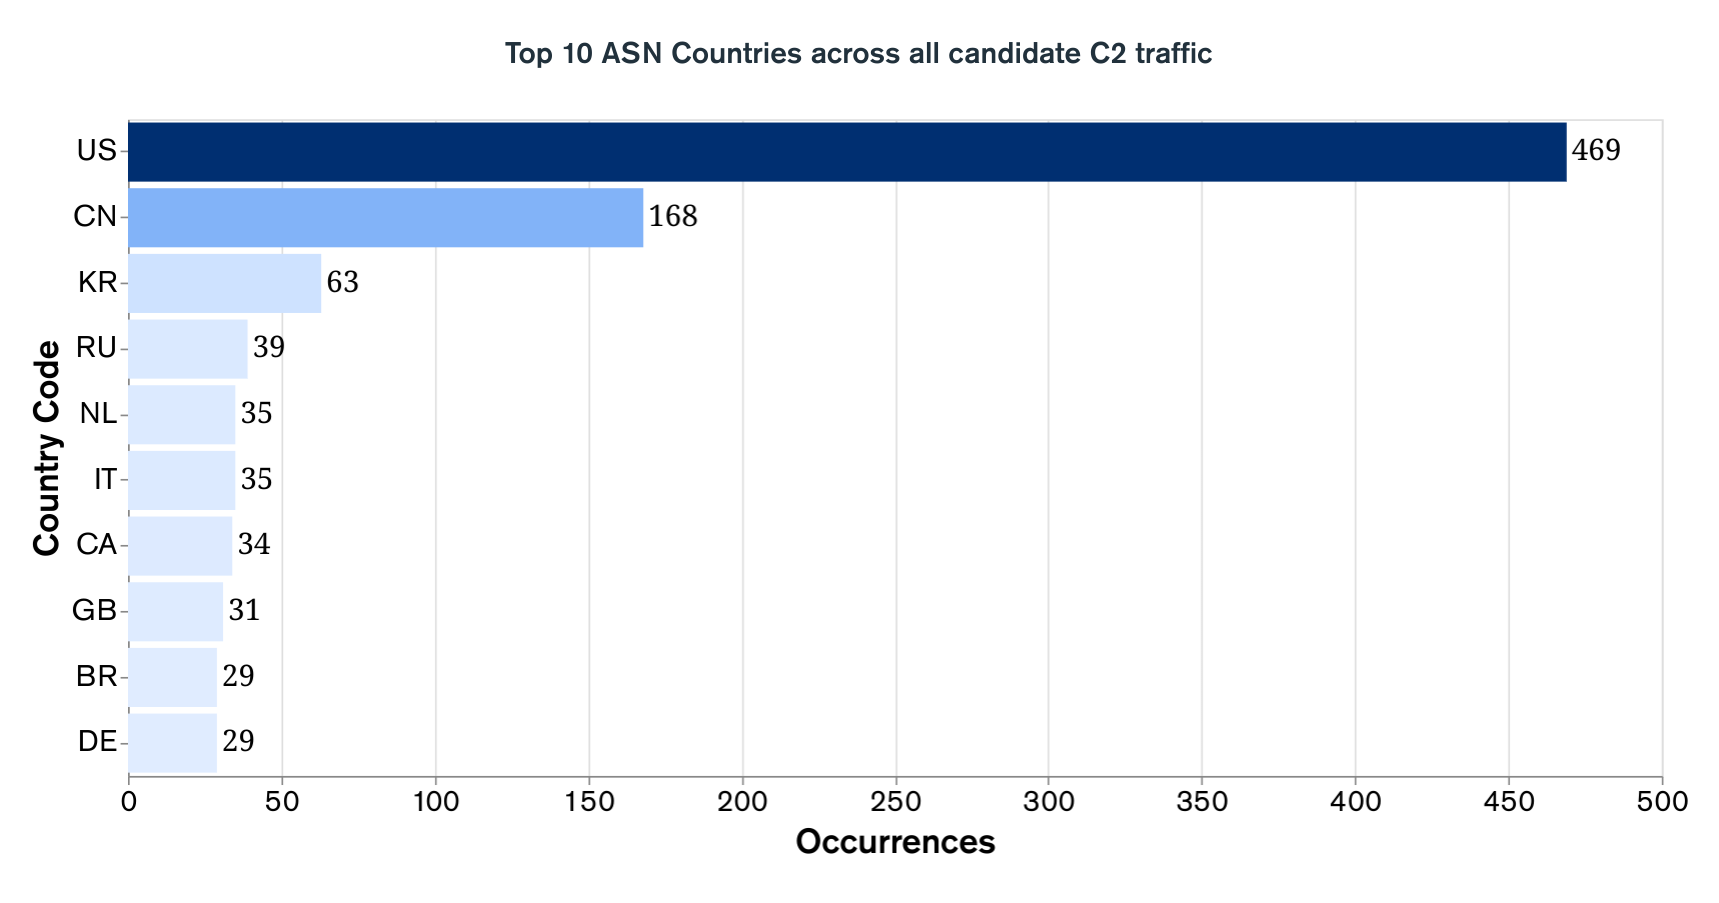
\includegraphics[width=6.55cm]{results/top_10_asn_countries_c2.png} }}
    \qquad
    \subfloat[\centering Top 10 P2P Node ASN Country Codes]{{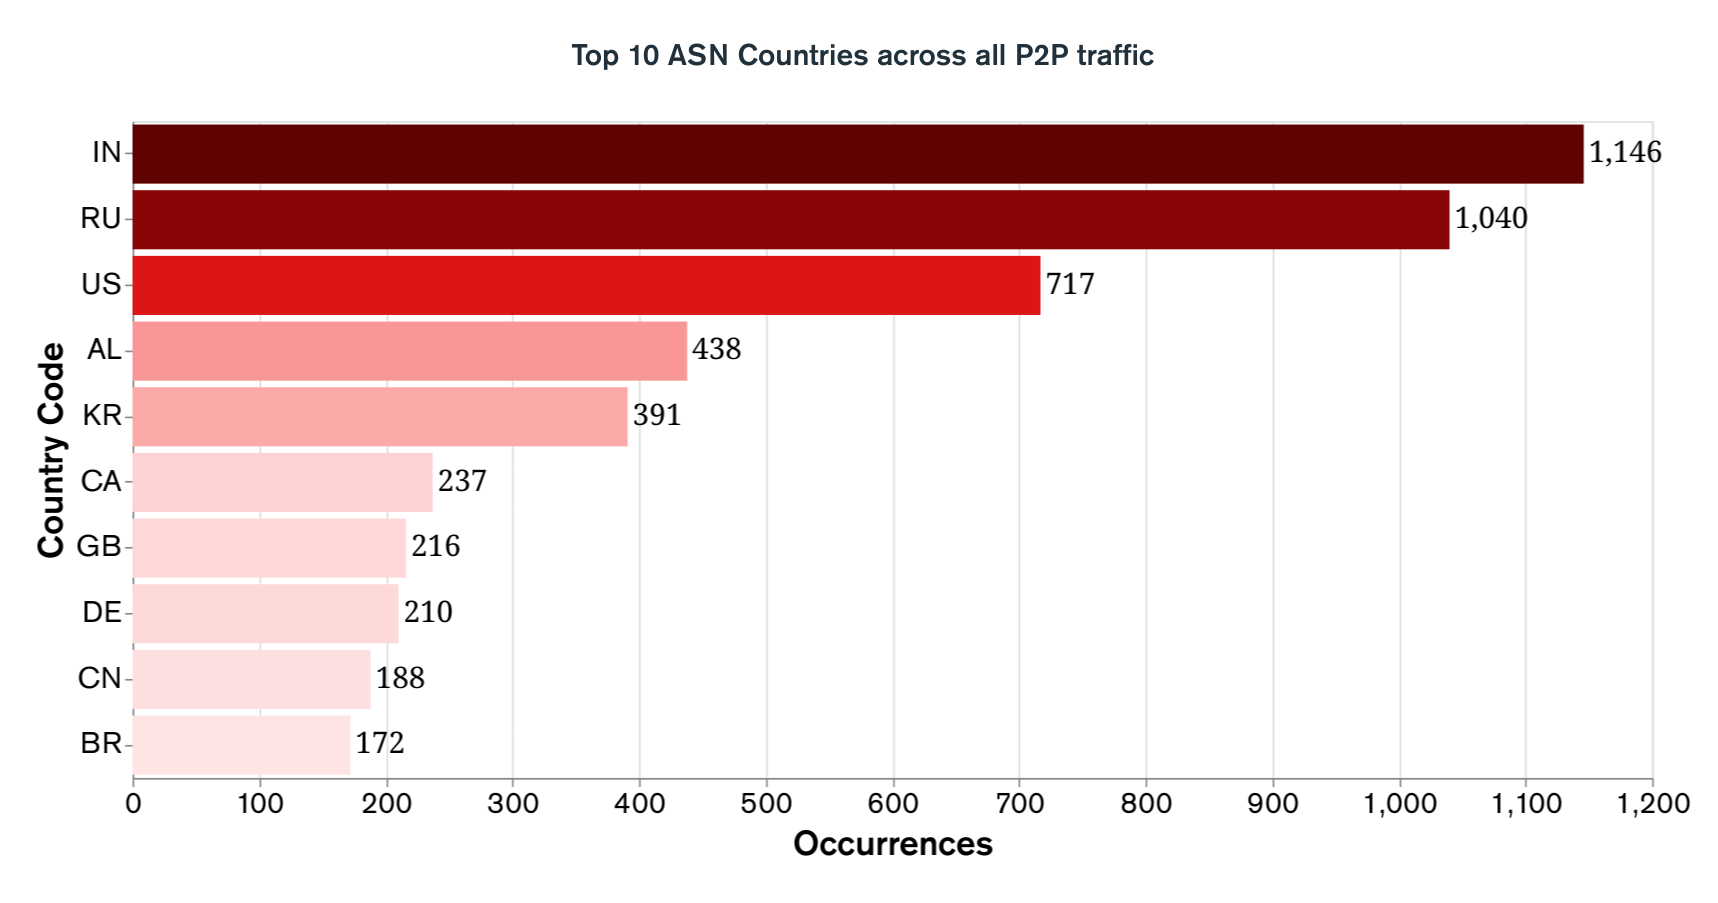
\includegraphics[width=6.55cm]{results/top_10_asn_countries_p2p.png} }}
    \caption{A side-by-side comparison of the geographic distribution of Autonomous Systems associated with P2P and C2 botnet activity.}
    \label{fig:p2p_c2_asn_dist}
\end{figure}

The above comparison illustrates a clear contrast between the distribution of C2, P2P, and overall traffic across the geographic regions of associated Autonomous Systems. The distribution of C2 ASN countries of origin confirms that most detected candidate C2 traffic originates from the United States. Contrary to that of C2 ASN distribution, logged Peer-to-Peer traffic predominantly originates from Autonomous Systems located in India, Russia, the United States, Albania, and South Korea, affirming that P2P botnet networks are more widely dispersed than that of C2 and propagation activity. Notably, most of the overall botnet traffic originates from IP addresses associated with AS4837 (China Unicom Backbone) and AS9829 (Bharat Sinchar Nigam Ltd.), located in China and India, respectively. The VisiBot Processing system also detected a significant amount of C2 botnet traffic originates from North American providers AS16625 (Akamai Technologies, Inc.) and AS16509 (Amazon.com). Diversely, the bulk of detected P2P traffic is more widely distributed across several ASNs, including AS8661 (Telekomi i Kosoves SH.A), AS9829 (Bharat Sinchar Nigam Ltd.), AS4766 (Korea Telecom), AS17465 (Asianet Satelite Communications), and AS12389 (Rostelecom). For the top 10 Autonomous Systems Numbers across C2, P2P, and overall botnet traffic, see Appendix \ref{appendix_a9}. 


\section{Traffic Analysis}

Despite a large proportion of benign botnet activity shown in Figure \ref{fig:botnet_distribution}, such as port-scanning activity, the second most commonly occurring traffic type is that of Peer-to-Peer Botnet traffic. As P2P nodes are identified during the malware analysis stage of the VisiBot Processing System, this indicates current popularity in the use of de-centralised Peer-to-Peer based infrastructures, like that of IoT botnets such as Hajime. Additionally, the number of packets classified as malicious botnet activity is significantly higher than that of identified payload and report server activity. The concept of a self-propagating malicious bot is a relatively new phenomenon amongst IoT botnet traffic, as such bots actively attempt to infect vulnerable devices using self-hosted malware. In comparison, conventional Mirai bots often report the detection of vulnerable devices to a report server, which performs remote code execution using malware hosted on a payload server. As self-hosted malware mitigates payload servers' requirement and allows for de-centralised propagation, this may explain why recently observed botnets utilise malicious bots more often than report or payload servers. 

In order to gain a better understanding the IoT devices which are currently being attacked, the VisiBot Processing System logs the detected packet categories and Common Vulnerability Exploits (CVEs) included within the packet information provided by the Bad Packets honeypot API. \citep{BadPackets} The below table represents the top 10 most commonly observed botnet packet categories and CVEs across all traffic classified by the VisiBot Processing System:

\begin{table}[!htb]
    \caption{Top 10 CVEs and packet categories across all botnet traffic}
    \centering
    \label{tab:cve_categories}
    \rowcolors{2}{}{gray!3}
    \begin{tabular}{|l|l|l|l|l|}
    \hline
    \textbf{CVE} & \textbf{Category} & \textbf{Description} & \textbf{Count} \\ \hline
    -               & Botnet Activity & Mirai-like Scan & 43,552 \\ \hline
    -               & IoT             & MVPower DVR (JAWS) RCE & 5,050 \\ \hline
    CVE-2016-10372  & Router          & Eir D1000 RCE & 1,878 \\ \hline
    -               & Router          & Netgear RCE & 632 \\ \hline
    CVE-2018-10561  & Router          & GPON RCE & 593 \\ \hline
    CVE-2016-6277   & Router          & Netgear RCE & 310 \\ \hline
    -               & IoT             & Vacron NVR RCE & 298 \\ \hline
    -               & IoT             & Generic CCTV-DVR RCE & 289 \\ \hline
    CVE-2013-7471   & Router          & D-Link UPnP SOAP RCE & 73 \\ \hline
    CVE-2013-3568   & Router          & Linksys RCE & 67 \\ \hline
    \end{tabular}
\end{table}

Botnet coordinators appear to be explicitly targeting IoT devices with known vulnerabilities through various attempts of Remote Code Execution (RCE). Malicious bots and/or report servers target devices such as routers, IP cams, and DVRs, all of which may be vulnerable to login credential brute-forcing attacks. Given the continued use of exploits known for a considerable amount of time, this indicates that there is still a significant amount of unpatched devices that attackers can infiltrate. Upon manual analysis of several attack packets collected by the honeypot, I observed that several infected devices were attempting to perform remote code execution using bash scripts hosted on remote payload servers. These bash scripts are used to ensure that the correct malware binary is executed on an infiltrated device, such that MIPS IoT devices are infected with a MIPS-compile binary and so on.


\section{Malware Analysis}

The previous observation of potential target CPU architectures is reaffirmed by the findings obtained through static analysis of several malware binaries collected during the data collection period of the VisiBot Processing System. As shown in figure \ref{fig:arch_vs_endianess}, static analysis of the extracted binaries collected by the VisiBot Processing System indicates that ARM and MIPS CPU architectures are currently being targeted at a high rate, with only 1.3\% of binaries targeting x86 devices. Similarly, botnets are mostly attacking IoT devices with big-endian memory addresses. This combined analysis indicates that the vast majority of detected traffic originates from IoT botnets, which explicitly target a wide range of devices distributed across two microprocessor architectures.

\begin{figure}[!htb]
    \centering
    \subfloat[\centering Malware Architecture]{{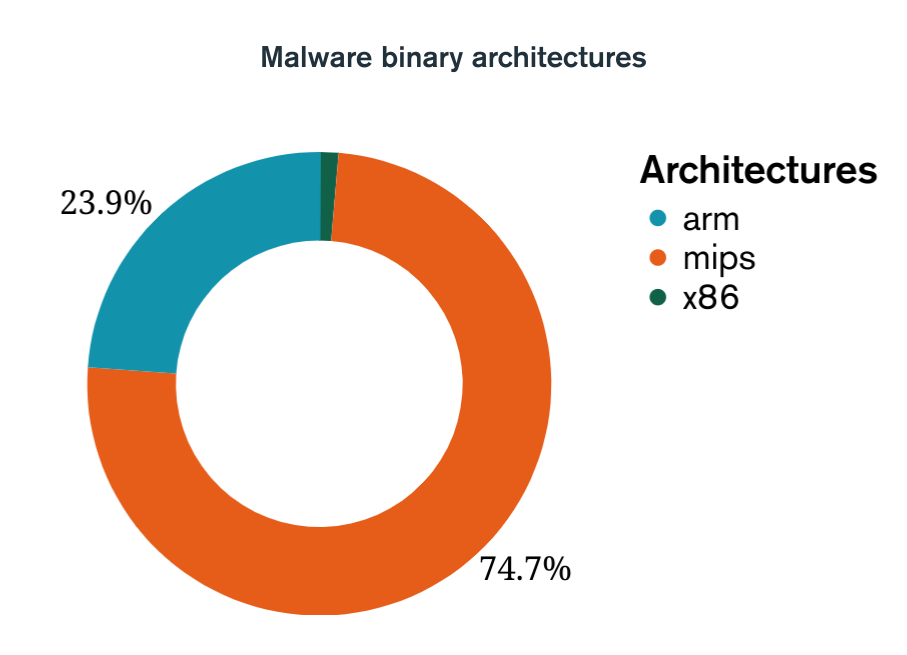
\includegraphics[width=6cm]{results/arch_piechart.png} }}
    \qquad
    \subfloat[\centering Malware Endianess]{{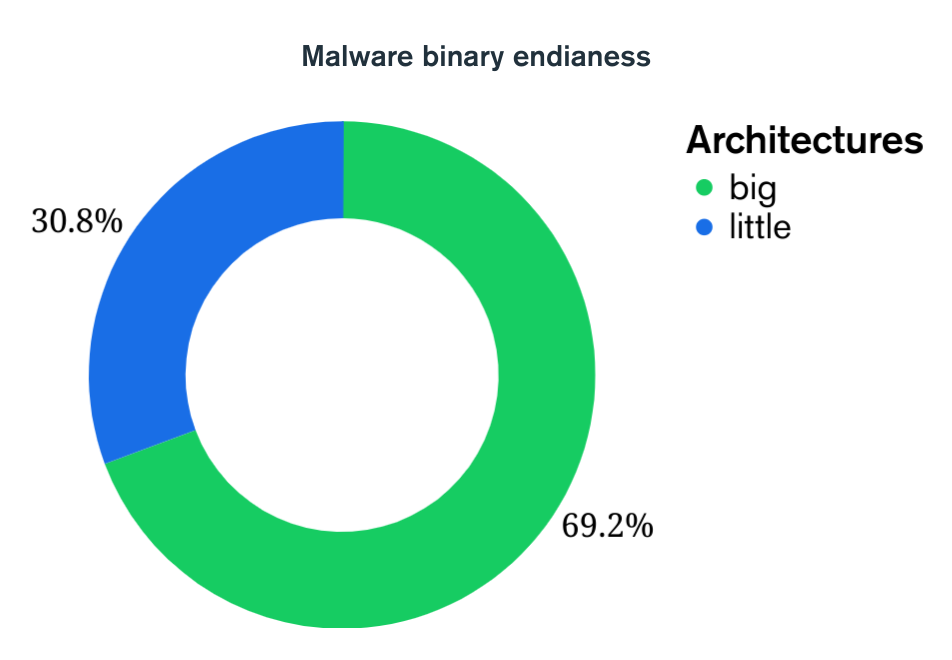
\includegraphics[width=6cm]{results/endianess_piechart.png} }}
    \caption{Malware sample architecture and endianess represented side by side.}
    \label{fig:arch_vs_endianess}
\end{figure}

Given these findings, it is likely that the types of botnets identified by the VisiBot are likely Mirai or Bashlite variants, as they are exclusively targeting IoT devices running on microprocessor technology. The distribution of identified botnet variants can be calculated by scanning each binary using VirusTotal and extracting the top-most occurring keyword across the positive vendor scan results. When a malware vendor positively identifies a binary as malicious, the malware's name is often characterised as a string, such as \texttt{Type:Platform/MalwareFamily}. As the result strings for positive vendor scans are given through the VirusTotal API, information such as the malware family can be parsed and sorted based on occurrence, such that keyword identifiers are extracted. The below table shows the most commonly occurring VirusTotal keywords across all analysed malware binaries:

\begin{figure}[!htb]
    \centering
    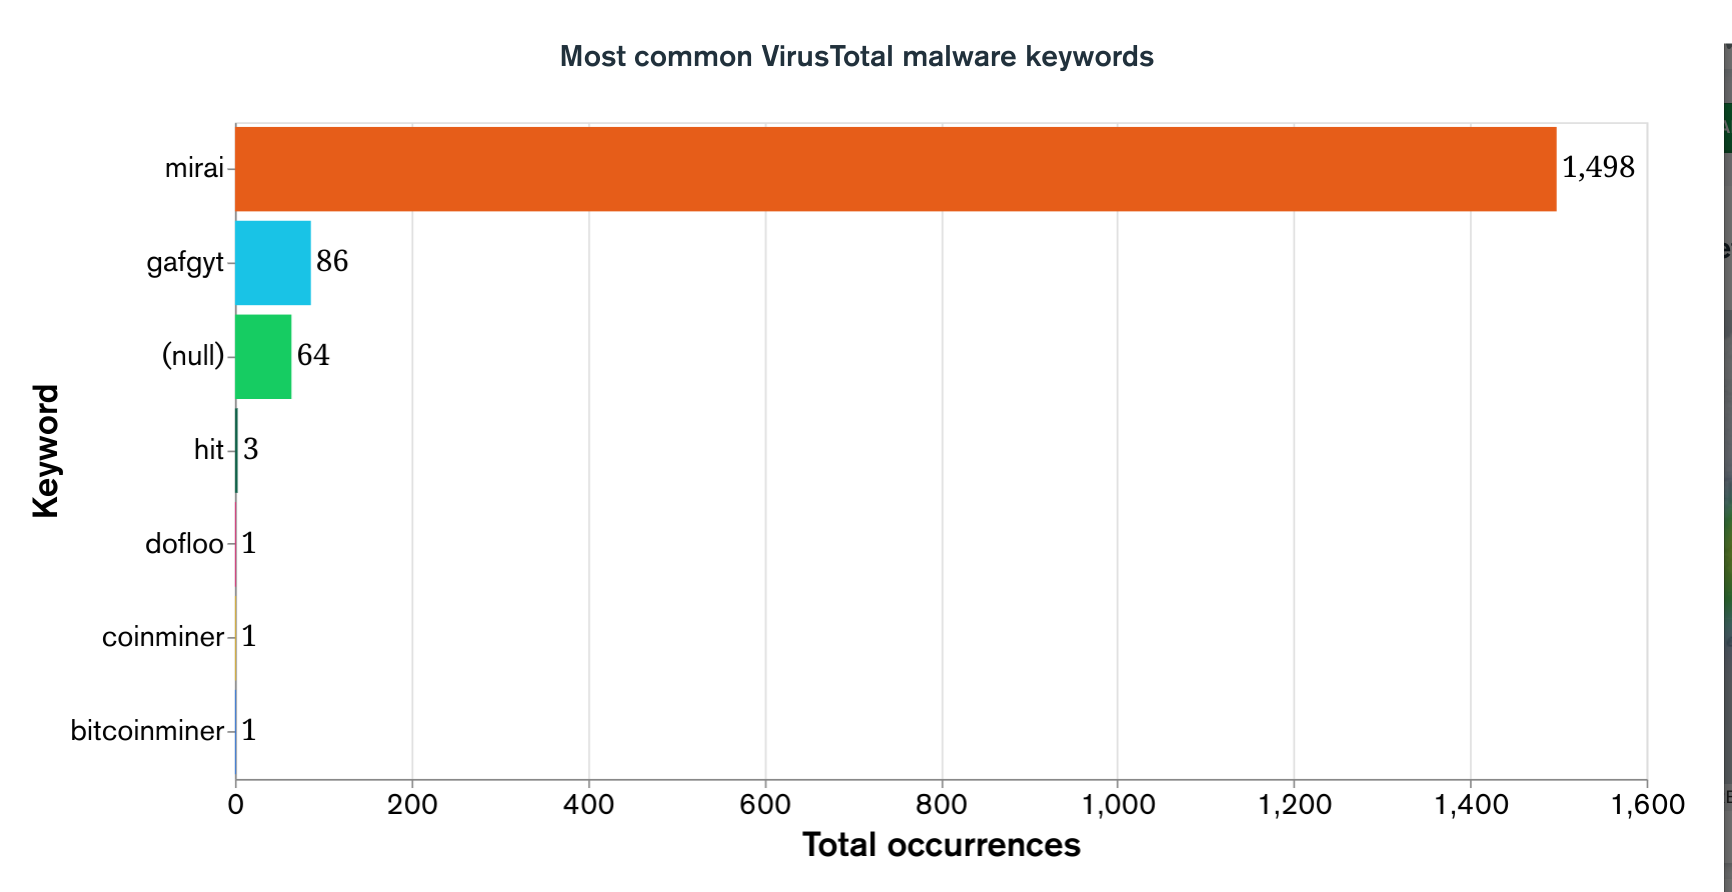
\includegraphics[width=0.75\linewidth]{results/vt_keywords.png}
    \caption{distribution of malware samples based on VirusTotal keywords}
    \label{fig:vt_keywords} 
\end{figure}

Although the vast majority of analysed binaries were detected as Mirai malware variants by the VirusTotal anti-virus vendors, some were identified as Bashlite (gafgyt) and coin-miners. The "hit" keyword in the above table is derived from the anti-virus result string \texttt{Trojan.Linux.Agent.HIT}. Despite testing positive, most VirusTotal anti-virus vendors could not detect the malware family of these binaries. Binaries that were not detected by the VirusTotal vendor scanning service were allocated the \texttt{(null)} placeholder keyword.


\subsubsection{Network Analysis}

During the network analysis stage of LiSa sandbox analysis, several network interactions originating from the infected sandbox host were logged, including all HTTP requests, DNS look-ups, and IRC Traffic. The logged HTTP requests were very typical to that of Mirai and Bashlite botnets, as several attempts were made by the infected host to brute-force and perform remote code execution on identified vulnerable devices. However, a significantly low number of DNS queries were observed throughout analysis of all 1,654 binaries, as a total of only 10 unique DNS look-ups were performed across all infected hosts:

\begin{table}[!htb]
    \centering
    \caption{Table of all DNS Queries logged during malware analysis}
    \label{tab:dns_queries}
    \rowcolors{2}{}{gray!3}
    \begin{tabular}{|c|c|c|c|c|}
    \hline
    \textbf{Domain} & \textbf{Record Type} & \textbf{Category} & \textbf{Total} \\ \hline
    dht.transmissionbt.com & A    & P2P DHT & 637 \\ \hline
    router.bittorrent.com  & A    & P2P DHT &  463 \\ \hline
    router.utorrent.com    & A    & P2P DHT &  452 \\ \hline
    bttracker.debian.org   & A    & P2P DHT &  441 \\ \hline
    jebiga.babyhub.pw      & A    & C2 Server &  6 \\ \hline
    hjar64zj6ygjd.com      & A    & C2 Server  &  2 \\ \hline
    cnc.fewbots.cc         & A    & C2 Server  &  1 \\ \hline
    g*y.energy             & A    & C2 Server  &  1 \\ \hline
    g*y.energy             & AAAA & C2 Server  &  1 \\ \hline
    ipinfo.io              & A    & Benign &  1 \\ \hline
    \end{tabular}
\end{table}

Notably, only four potential Command \& Control server DNS recorders were identified, with most DNS lookups being associated with public Peer-to-Peer services and Distributed Hash Tables. Of the C2 DNS records identified, one domain name shows low vowel density and high Sharron entropy (randomness), common to that of conventional Mirai C2 domain names. \citet{Dwyer2019} However, as shown,  DNS based botnet detection would not have proved beneficial in this case as a small number of DNS lookups were observed. The querying of public P2P service domains is a relatively innovative characteristic of de-centralised IoT botnets, such as Hajime or Mozi. Once a bot is infected, it will attempt to access the botnet DHT through public BitTorrent services, such as those logged above. Such DNS queries were previously observed in Mozi botnet network activity by \citep{Netlab2019}. A high occurrence of Mozi malware amongst collected binaries can be observed in the word cloud generated in Appendix \ref{appendix_a8}, validating that a large proportion of the botnet traffic detected by the VisiBot Processing System originates from the Mozi botnet. The filenames \texttt{Mozi.a} and \texttt{Mozi.m} also signify devices running on \textbf{a}rch and \textbf{m}ips CPU architectures are being directly targeted by Mozi. 

\subsubsection{Malware Port Usage}

The UDP and TCP network statistics are shown in Appendix \ref{appendix_a7} also reaffirms that the majority of detected botnet traffic is specific to the targeting of IoT, as devices are primarily targeted via Telnet (22/2323) and HTTP (80) via the TCP protocol. As many IoT devices have vulnerabilities in online dashboards, attackers often attempt credential brute-forcing and remote code execution (RCE) exploits on IoT dashboards/panels accessible through port 80. Other highly targeted TCP ports, such as 5555, 49152, and 37215, are ports commonly used by IoT devices such as IP cameras and routers. Highly targeted ports, such as 7574, are associated with cluster services such as the Oracle Coherence Cluster service, indicating that attackers may be actively trying to infiltrate cluster systems using known exploits. Notably, ports 443 and 22, commonly used with HTTPS and SSH, are very low on the list of targeted TCP ports. This suggests that attackers are less concerned with the brute-forcing of SSH clients and routing of traffic through secure network layers such as HTTPS.

In contrast to TCP, the UDP ports 67, 1900, 53, and 6881 were also largely targeted by bots observed throughout malware sandbox analysis. The UDP port 53 is often listened to by worms and botnets awaiting incoming commands from the C2 servers. \citep{SpeedguidePort53} Whereas, ports 67 and 1900 are typically used by DHCP servers and UPnP devices, as highlighted in Table \ref{tab:cve_categories}. However, the vast majority of logged UDP traffic (shown in Figure \ref{fig:udp_port_stats}) is widely and randomly distributed across various ports. These unusual characteristics may be an indication of malicious bot activity associated with Mozi botnets. Mozi bots propagate the botnet through self-hosting malware on local webservers hosted at randomly selected UDP ports. The files hosted on the temporary webserver are downloaded when the malicious bot successfully brute-forces or performs remote code execution on a vulnerable IoT device. After some time, the port of the webserver changes to a different randomly selected port. The presence of such activity may explain why a high number of malware payload URLs were extracted from detected honeypot packets. Still, only a small percentage of binaries were retrievable. It is possible that the VisiBot Processing System wasn't quick enough in retrieving malware binaries from certain URLs. This issue may be caused by the limitation of having to query the honeypot service used by VisiBot on an hourly basis. Should packets be processed immediately upon identification, it is likely that the URL pointing to a randomly selected port will still be active, allowing for a higher number of samples to be collected.

\subsubsection{P2P Payload Connections Analysis} Generated using NetworkX \citep{NetworkX} and the K-Components approximation algorithm \cite{NetworkXKComponents}, the below edge-connectivity graph visualises the various relationships between analysed malware binaries and identified Peer-to-Peer networks using the IP address connection relationship information logged throughout network analysis of analysed malware binaries:

\begin{figure}[!htb]
    \centering
    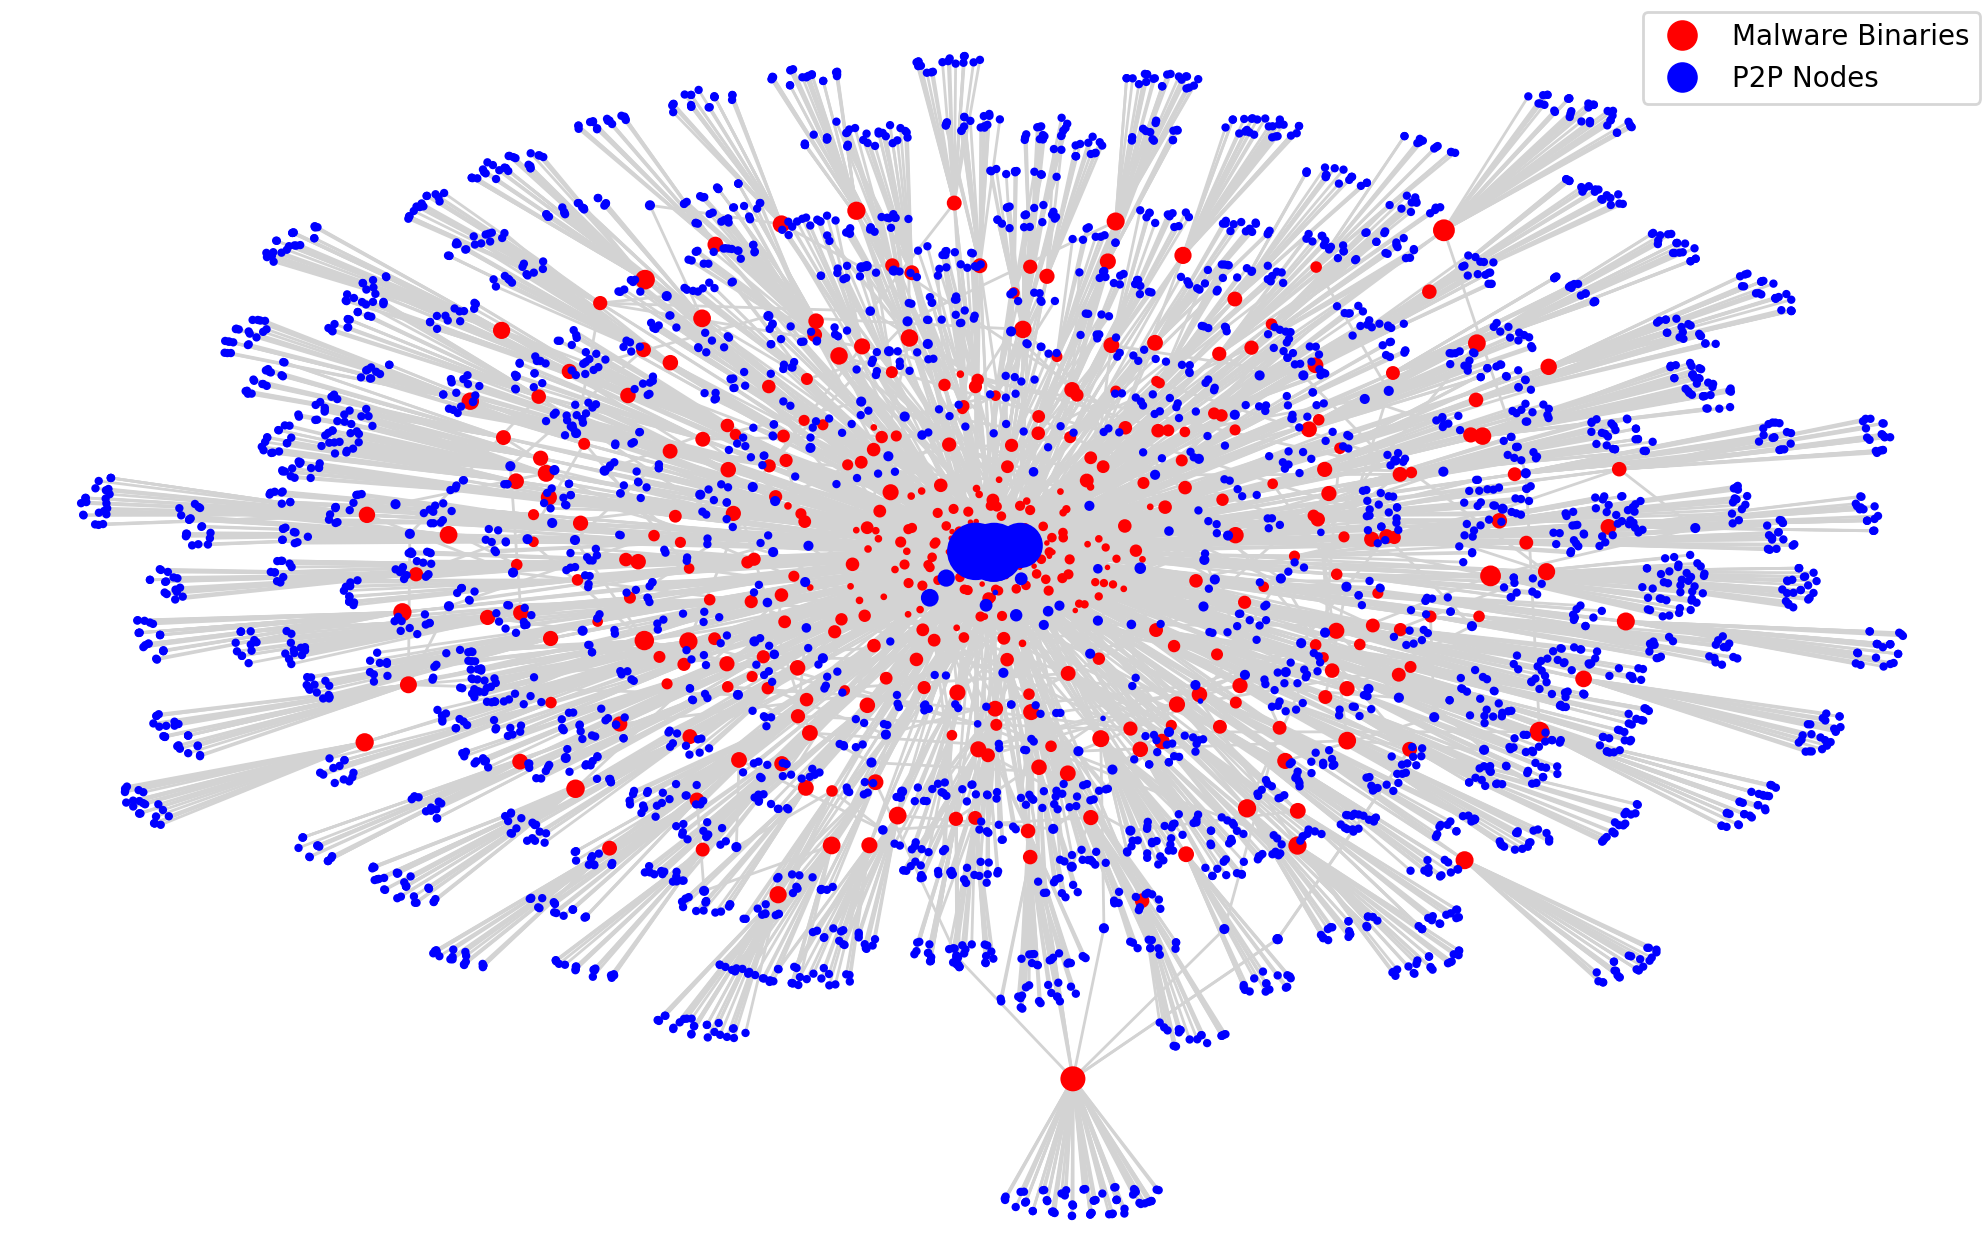
\includegraphics[width=0.95\linewidth]{results/p2p_payload_network.png}
    \caption{Edge-connectivity graph of P2P Node and malware binary interactions recorded during network analysis. Edge connections approximated using K-Components algorithm.}
    \label{fig:p2p_payload_networks} 
\end{figure}

Several small-scale Peer-to-Peer botnets are shown throughout the perimeter of the graph, with several P2P networks being interlinked through some mediary P2P nodes. As shown, various of the small-scale P2P networks detected during analysis are interlinked with each other, and with larger P2P networks spanning across the centre of the graph. The blue mass of Peer-to-Peer nodes at the centre of the visualisation indicates botnet propagation growth of one or more large P2P botnets over the 5-week data collection period, as several connections between P2P nodes have been established across multiple payload binaries which are likely to originate from the same botnet. However, as public distributed hash tables are often used in Peer-to-Peer botnets, it is likely that a high proportion of this traffic is legitimate, as bots often interact with legitimate peers to throw-off potential network analysis. \citep{Herwig2019} A summary of the number of nodes associated with malware payloads is shown below:

\begin{table}[!htb]
    \centering
    \caption{Summary: Number of P2P Nodes identified during malware binary analysis.}
    \label{tab:p2p_payload_summary}
    \rowcolors{2}{}{gray!3}
    \begin{tabular}{|c|c|c|c|c|c|}
    \hline
    \textbf{Min} & \textbf{1st Quartile} & \textbf{Median} & \textbf{Mean} & \textbf{3rd Quartile} & \textbf{Max} \\ \hline
    1.0 & 5.0 & 12.0 & 12.75 & 18.0 & 69.0 \\ \hline
    \end{tabular}
\end{table}

\subsubsection{Candidate C2 Server ASN History Analysis} The relationships between identified candidate C2 servers and Autonomous Systems are also visualised using the same K-Components approximation algorithm used above. Using  the recent ASN history of all candidate C2 Servers, sourced from various WHOIS records via ipwhois \citep{ipwhois}, the below network graph illustrates the historical interactions, such as ownership or temporary holdings, between Autonomous Systems and identified candidate C2 servers:

\begin{figure}[!htb]
    \centering
    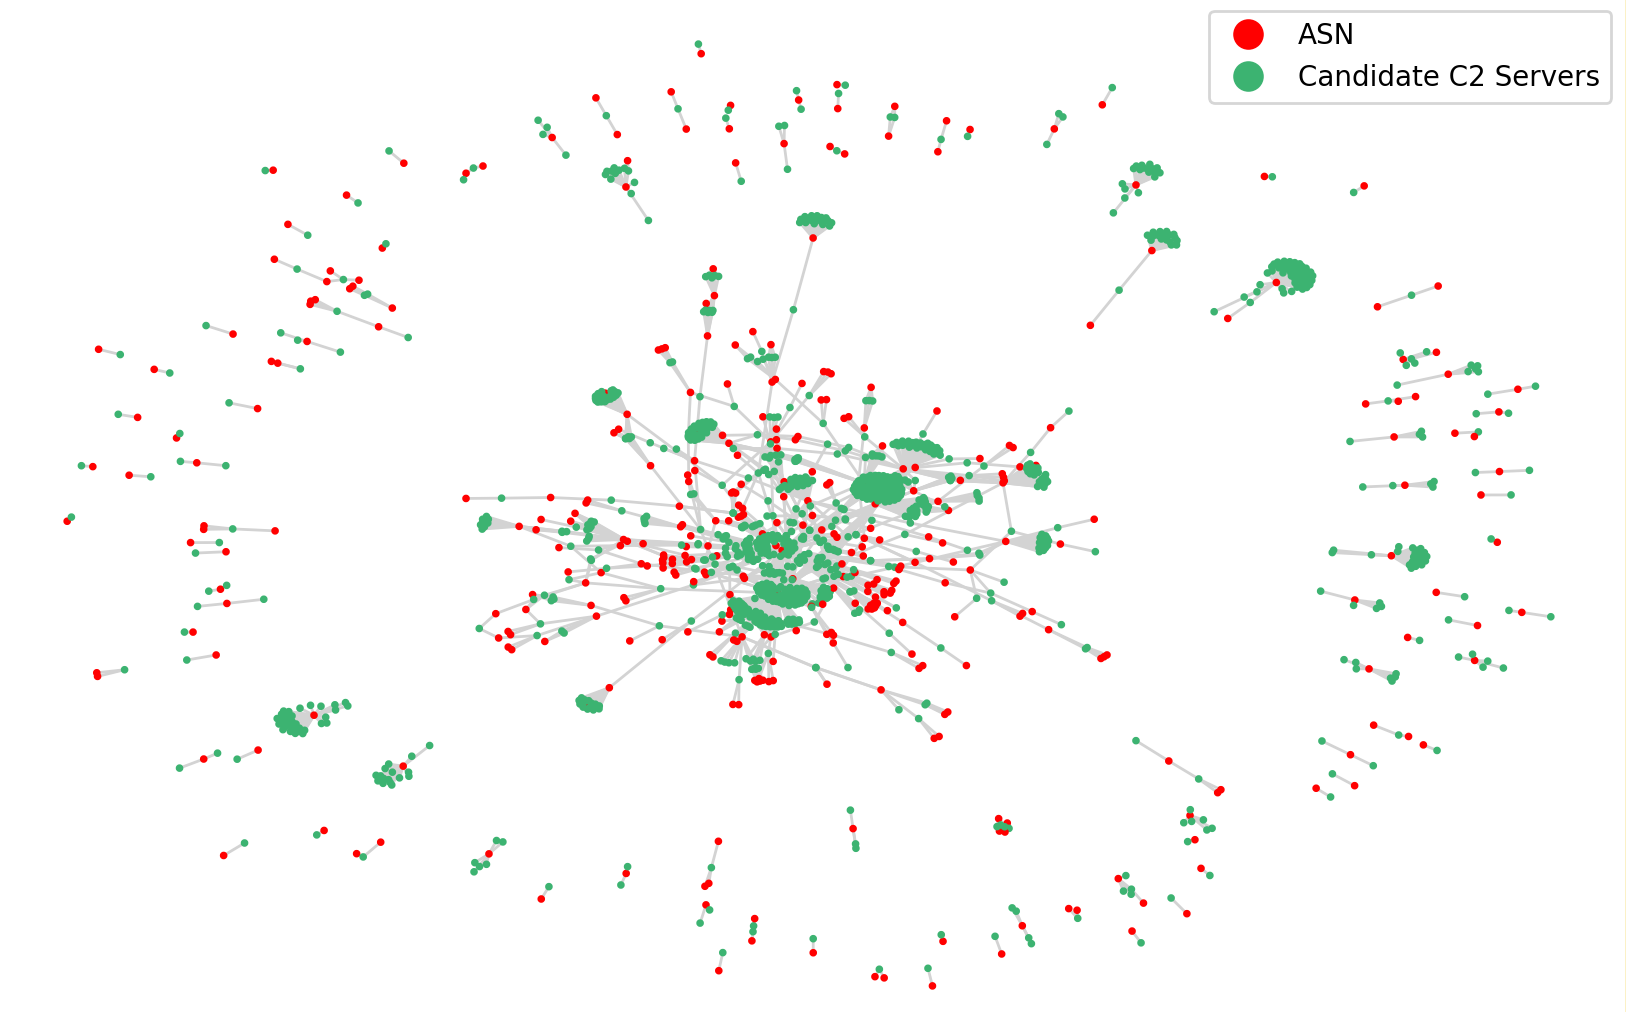
\includegraphics[width=0.9\linewidth]{results/c2_asn_network.png}
    \caption{Edge-connectivity graph of P2P Node and malware binary interactions recorded during network analysis. Edge connections approximated using K-Components algorithm.}
    \label{fig:c2_asn_networks} 
\end{figure}

\begin{table}[!htb]
    \centering
    \caption{Summary: Number of ASNs associated with 1,157 candidate C2 Servers}
    \label{tab:c2_asn_history_summary}
    \rowcolors{2}{}{gray!3}
    \begin{tabular}{|c|c|c|c|c|c|}
    \hline
    \textbf{Min} & \textbf{1st Quartile} & \textbf{Median} & \textbf{Mean} & \textbf{3rd Quartile} & \textbf{Max} \\ \hline
    1.0 & 3.0 & 5.0 & 5.437 & 9.0 & 10.0 \\ \hline
    \end{tabular}
\end{table}

As shown above, the central network cluster indicates that several ASNs are holding/exchanging ownership of IP addresses associated with Command \& Control activity detected by VisiBot. Additionally, it is observed that a high number of C2 IP addresses are owned by a select few Autonomous Systems, with a mean average of 5 ASNs associated with identified candidate Command \& Control servers. An iterative graph-based monitoring tool can be built using this information to observe the interactions between C2 Servers and ASNs. Such observations may allow for insight into the trading/holding process of IP addresses associated with botnet activity amongst Autonomous Systems.


\section{Evaluation}

Over a 35-day experimentation period, the distributed honeypot system, automated malware extraction, and botnet classification processes employed by VisiBot enabled the detection of over 58,010 unique IP addresses and the collection of 1,654 malware samples comprised of 150 unique MD5 hashes over 35 days. In comparison, the IoTPoT honeypot system proposed by \citet{PaPa2016} identified a total of 16,934 visiting IP addresses and collected 43 unique malware samples over a 39-day evaluation period. The significant difference in the number of unique IP addresses encountered highlights the advantages of using a strategically distributed honeypot network. The extensive, worldwide, and intelligent honeypot services provided by \citet{BadPackets} permitted the processing of thousands of honeypot packets per day, enabling the significantly higher collection of malware samples over a shorter evaluation period.

Given the significant number of malware URLs extracted during the experimentation period, the payload URL extraction employed by VisiBot has proven highly effective. The combination of regular expression pattern matching and manual re-building of URLs obfuscated using command-line arguments allows for the efficient and computationally inexpensive identification of sample URLs used in botnet remote code execution attacks. However, a considerable proportion of the extracted malware URLs were no longer active upon reaching the malware analysis stage. Out of the 9,923 URLs identified, only 1654 malware samples were collected due to limitations within the honeypot collection process.

During the 35-day experimentation period, VisiBot encountered a significant number of malicious bots originating from the Mozi botnet variant, which were observed to be performing remote code execution attacks using self-hosted malware samples. However, as the corresponding port for hosting malware is frequently changed, a small window of time is given to download the binary before the URL expires. As the VisiBot Processing System retrieves honeypot data on an hourly basis from an external honeypot service, the hour-long delay between intrusion detection and analysis often results in such malware URLs expiring before binaries can be downloaded and analysed. A possible solution is to use a real-time stream or socket-based honeypot API, allowing packets to be analysed within a short time frame of being detected by a given honeypot. By doing so, a more significant proportion of self-hosted payload URLs can be collected.

Implementing a scalable and distributed sandbox analysis system allows for automatic static, dynamic and network analysis of malware samples extracted from the honeypots utilised by VisiBot. In doing so, the VisiBot Processing System was able to identify significant botnet traffic following the heuristic analysis of 1318 out of 1654 malware binaries, yielding an identification rate of 79.87\%. Opposed to these results, the botnet detection techniques and heuristics employed by \citet{Bastos2019} permitted the C2 server detection of 1010 out of 1050 malware samples, resulting in a detection rate of 96\% across all samples. However, both systems are comparably quite different.  The method proposed by \citet{Bastos2019} is exclusively concerned with the identification of Centralised Command \& Control servers from the conventional IoT botnets, Mirai and Bashlite. It does not consider approaches for identifying de-centralised botnets. Whereas the VisiBot Processing System is primarily concerned with identifying both centralised and de-centralised IoT Botnets, allowing for the detection of C2 servers and Peer-to-Peer botnet traffic generated by relatively new botnet variants such as Mozi and Hajime.

Nevertheless, one significant drawback of the VisiBot Processing System, in its current state, is that there is no validation process in place for confirming the validity of identified candidate C2 and P2P traffic through the likes of executing hand-shaking procedures. Many de-centralised botnets communicate with legitimate public Peer-to-Peer networks, and centralised botnets are known to communicate with fake C2 servers to mislead authorities. Thus, the legitimacy of the C2 or P2P candidates identified by VisiBot should be assumed, as such entities must first be validated through the invocation of several botnet handshake procedures. Through performing handshakes with candidate C2 servers, the legitimacy of each C2 can be inferred based on the handshake response from its server. However, this functionality is not yet present within the VisiBot Processing System but can be extended in future iterations to include such validation procedures.

A considerable number of candidate C2 servers and P2P Nodes were detected through the VisiBot Processing System, indicating that the chosen heuristics effectively differentiate between benign and malicious botnet traffic. However, the lower detection rate indicates when compared to other systems suggests that some of the heuristics used were less effective than anticipated. A high number of packed malware binaries were observed during the data collection period. Botnet owners were primarily using the UPX packing tool \citep{UPX} to compress binaries and obfuscate source code. Despite making modifications to the LiSa sandboxing server to enable the unpacking of UPX binaries, many samples could not be successfully unpacked. This resulted in the collection of obfuscated binary strings during static analysis, which proved too noisy for extracting hard-coded IP addresses. Following this, the heuristic-based detection of connections to hard-coded IP addresses proved the least effective across all four heuristics. However, with further improvements to binary un-packing procedures, this heuristic will likely prove more advantageous for identifying candidate Command \& Control servers.

Throughout the 35-day data collection period, the VisiBot Processing System has proven highly reliable and robust, having automated extensive analysis procedures for over 61,000 honeypot events. The logging of botnet entity interactions, traffic classifications, sample analysis information, geographic data, and autonomous system history allows for many insights to be made regarding the current state and potential evolutionary patterns of IoT Botnets. The collection and analysis of malware binaries has proven effective in identifying the source of control amongst centralised and de-centralised botnets. However, analysis of target binary CPU architectures and frequently observed Common Vulnerability Exploits also give insight into how IoT botnets are propagating and the types of exploit mechanisms that botnet developers are employing. Graph-based visualisations of C2 and Autonomous System interactions also provide insight into the interplay between Autonomous Systems and botnet IP addresses. The visualisation of Peer-to-Peer connections observed between malware payloads also can be used to measure the rate at which such botnets are propagating. Additionally, visualisations can assist with identifying centralised interactions between P2P node IP addresses. Collectively, the variety of information collected by the VisiBot Processing System is highly significant within Cyber Threat Intelligence.